\chapter{Linear Models: Multiple explanatory variables}
\label{ch:MulExpl}

Aims of this chapter\footnote{Here you work with the script file {\tt MulExpl.R}}:

\begin{compactitem}
	\item Including several explanatory variables in a model
	\item Interpreting summary tables for more complex models
\end{compactitem}

\section{Loading the data}

\begin{compactitem}[$\quad\star$]
	\item Create a new blank script called {\tt MulExpl.R} in your 
	{\tt Code} directory and add some introductory comments.

	\item Use {\tt load('../Data/mammals.Rdata')} to load the data saved 
	at the end of Chapter~\ref{ch:ANOVA}. Look back at the end of Chapter 
	\ref{ch:ANOVA} to see how you saved the RData file. If {\tt 
	mammals.Rdata} is missing, just import the data again using {\tt 
	read.csv("../Data/MammalData.csv")} and add the log C Value column to 
	the imported data frame again (got back to Chapter~\ref{ch:ANOVA} and 
	have a look if you have forgotten how).

	\item Use {\tt ls} and {\tt str} to check that the data has loaded 
	correctly.
	
\end{compactitem}

The models we looked at in Chapter~\ref{ch:ANOVA} explored whether 
the log genome size (C value, in picograms) of terrestrial mammals 
varied with trophic level and  whether or not the species is ground 
dwelling. We will now look at a single model that includes both 
explanatory variables. 

The first thing to do is look at the data again. In Chapter 
\ref{ch:regress}, we asked if carnivores or herbivores had larger 
genomes. Now we want to ask questions like: do ground-dwelling 
carnivores have larger genomes than arboreal or flying omnivores? We 
need to look at plots within groups. 

Before we do that, there is a lot of missing data in the data frame and 
we should make sure that we are using the same data for our plots and 
models. We will subset the data down to the complete data for the three 
variables:

\begin{lstlisting}
> mammals <- subset(mammals, select = c(GroundDwelling, TrophicLevel, 
logCvalue))
> mammals <- na.omit(mammals)
> str(mammals)

'data.frame':	259 obs. of  3 variables:
 $GroundDwelling: Factor w/ 2 levels "No","Yes": 2 2 2 2 2 1 2 1 1 1 ...
 $TrophicLevel  : Factor w/ 3 levels "Carnivore","Herbivore",..: 1 2 2 2 3 3 3 2 2 3 ...
 $logCvalue     : num  0.94 1.322 1.381 1.545 0.888 ...
  - attr(*, "na.action")=Class 'omit'  Named int [1:120] 2 4 7 9 10 11 14 15 20 21 ...
   .. ..- attr(*, "names")= chr [1:120] "2" "4" "7" "9" ...
\end{lstlisting}

\section{Boxplots within groups}

In Chapter~\ref{ch:regress}, we used the {\tt subset} option to fit a model just to 
dragonflies. You can use {\tt subset} with plots too.

\begin{compactitem}[$\quad\star$]
	\item Add {\tt par(mfrow=c(1,2))} to your script to split the 
	graphics into two panels.
	\item Copy the code from Chapter~\ref{ch:ANOVA} to create a boxplot 
	of genome size by trophic level into your script.
	\item Using this, and adding a {\tt subset} option to the code, 
	generate the plots shown in the figure below.
	\item You can use the option {\tt main} to add titles to a plot.
\end{compactitem}

\begin{center}
	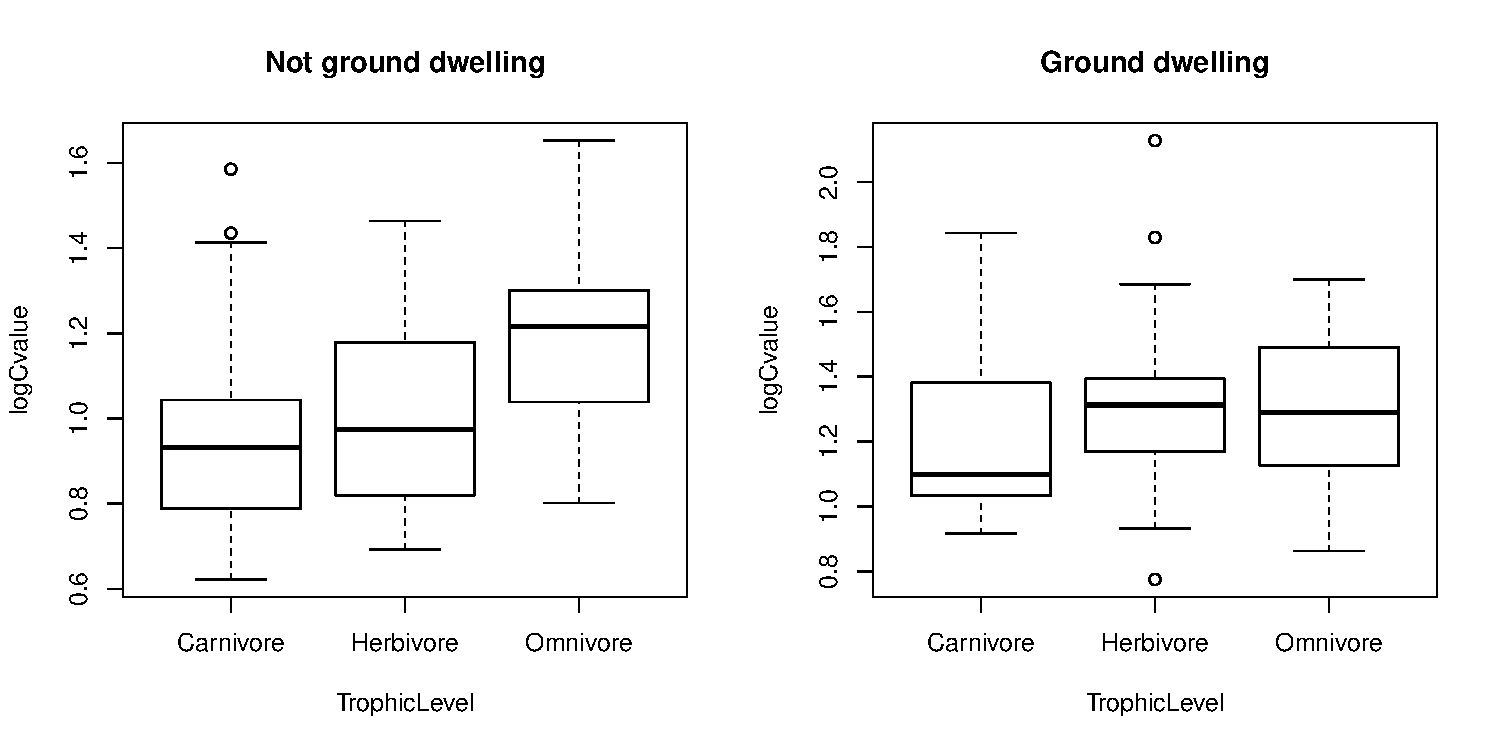
\includegraphics[width=1.0\textwidth]{boxplots.pdf}
\end{center} 

\section{{\tt lattice} again}

Recall that the {\tt lattice} package provides some very neat extra 
ways to plot data in groups. They look pretty but the downside is that 
they don't use the same graphics system --- all those {\tt par} 
commands are useless for these graphs. The defaults look good though!

\begin{lstlisting}
> library(lattice)
> bwplot(logCvalue ~ TrophicLevel | GroundDwelling, data= mammals)
\end{lstlisting}

\begin{center}
	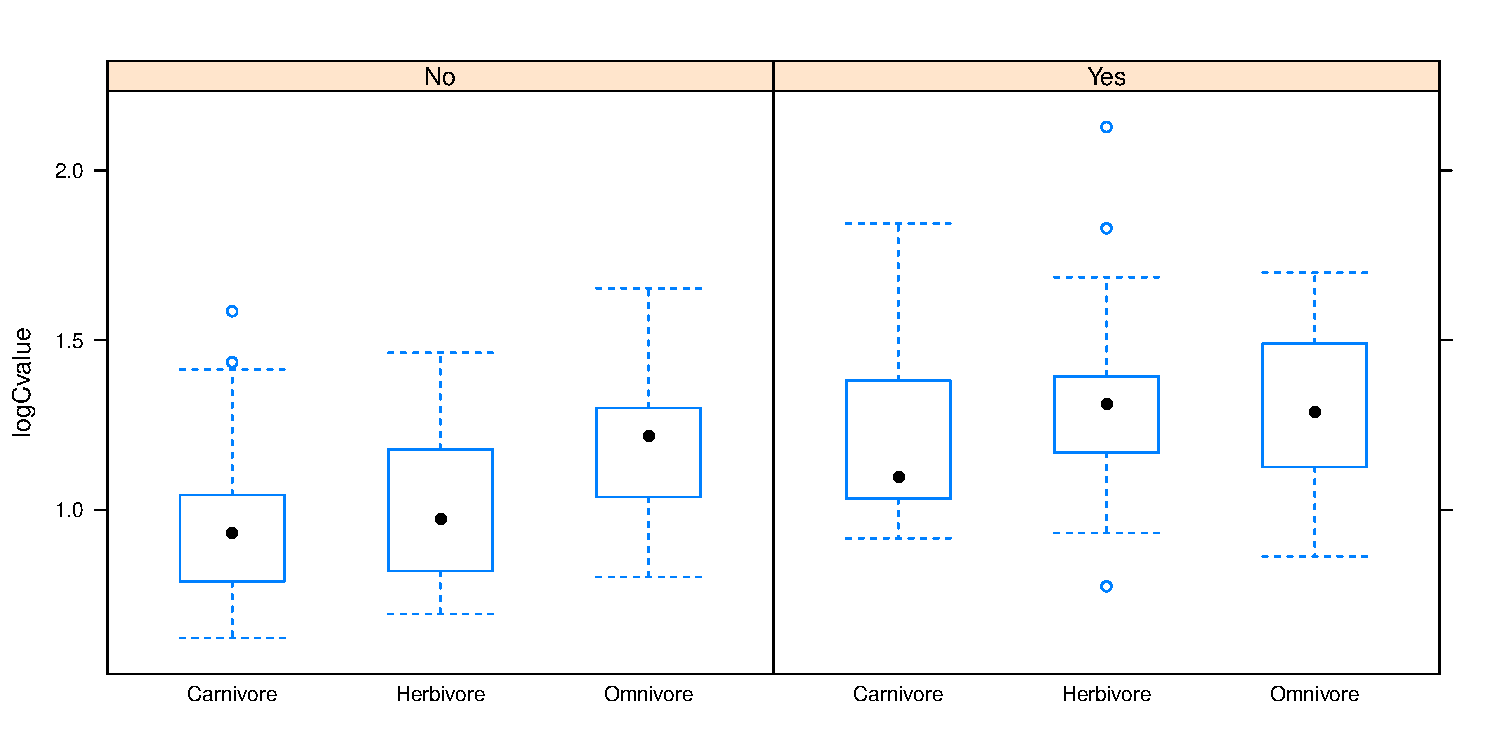
\includegraphics[width=1.0\textwidth]{bwplots.pdf}
\end{center}
	
The code {\tt logCvalue \textasciitilde{} TrophicLevel | 
GroundDwelling} means plot the relationship between genome size and 
trophic level, but group within levels of ground dwelling. We are using 
the function {\tt bwplot}, which is provided by {\tt lattice} to create 
box and whisker plots. 

\begin{compactitem}[$\quad\star$]
	\item Create the lattice plots above from within your script.
	\item Rearrange this code to have three plots, showing the box and 
	whisker plots for {\tt GroundDwelling}, grouped within the levels of 
	{\tt TrophicLevel}.
	\item Try reshaping the R plot window and running the command again. 
	Lattice tries to make good use of the available space when creating 
	lattice plots.
\end{compactitem}

\section{Barplots again}

We're going to make the barplot code from Chapter~\ref{ch:regress} even more 
complicated! This time we want to know the mean log genome size within 
combinations of {\tt TrophicLevel} and {\tt GroundDwelling}. We can 
still use {\tt tapply}, providing more than one grouping factor. We 
create a set of grouping factors like this:


\begin{lstlisting}
> groups <- list(mammals$GroundDwelling, mammals$TrophicLevel)
> groupMeans <- tapply(mammals$logCvalue, groups, FUN = mean)
> print(groupMeans)

     Carnivore Herbivore Omnivore
 No     0.9589     1.012    1.192
 Yes    1.2138     1.298    1.299
\end{lstlisting}

\begin{compactitem}[$\quad\star$]
	\item Copy this code into your script and run it.
	\item Use this code and the script from Chapter~\ref{ch:ANOVA} to get the set of 
	standard errors for the groups({\tt groupSE}). You should get this: 
\end{compactitem}

\begin{lstlisting}
     Carnivore Herbivore Omnivore
 No    0.04842   0.03419  0.02410
 Yes   0.05976   0.02787  0.03587
\end{lstlisting}

Now we can use {\tt barplot}. The default option for a barplot of a 
table is to create a stacked barplot, which is not what we want. The 
option {\tt beside=TRUE} makes the bars for each column appear side by 
side. Once again, we save the midpoints of the bars to add the error 
bars. The other options in the code below change the colours of the 
bars and the length of error bar caps.
% 
\begin{lstlisting}
	# get upper and lower standard error height
> upperSE <- groupMeans + groupSE
> lowerSE <- groupMeans - groupSE

# create barplot
> barMids <- barplot(groupMeans, ylim=c(0, max(upperSE)), beside=TRUE, 
ylab= ' log C value (pg) ' , col=c( ' white ' , ' grey70 '))

> arrows(barMids, upperSE, barMids, lowerSE, ang=90, code=3, len=0.05)
\end{lstlisting}

\begin{center}
	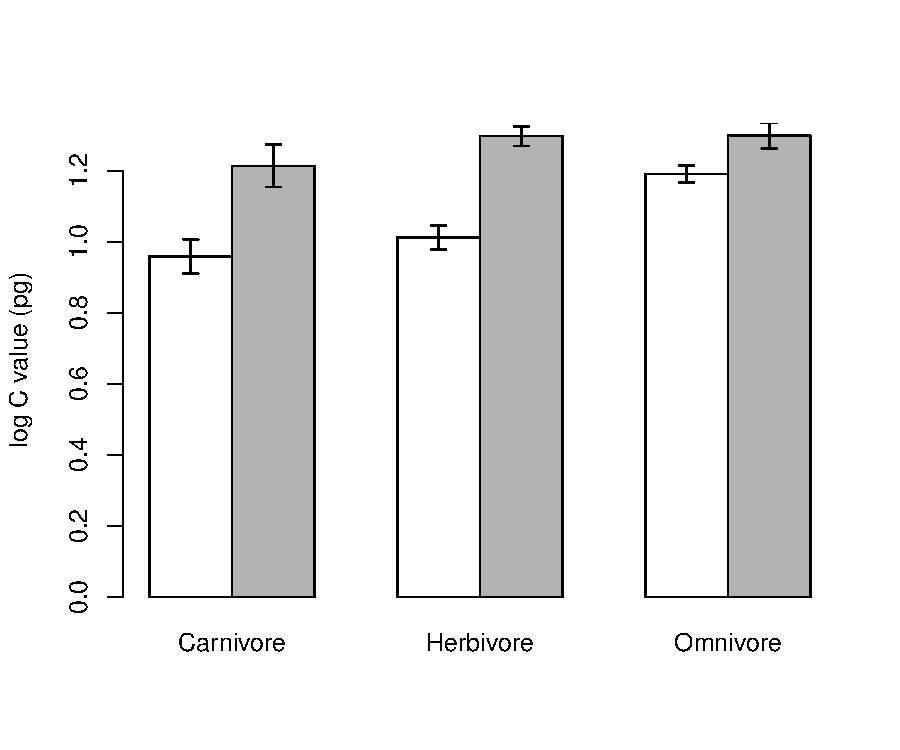
\includegraphics[width=0.6\textwidth]{barplot_1.pdf}
\end{center} 

\begin{compactitem}[$\quad\star$]
	\item Generate the barplot above and then edit your script to change 
	the colours and error bar lengths to your taste.
\end{compactitem}

\section{Plotting means and confidence intervals}

We'll use the {\tt plotmeans} function again as an exercise to change 
graph settings and to prepare figures for write ups. 

\begin{figure} \centering 
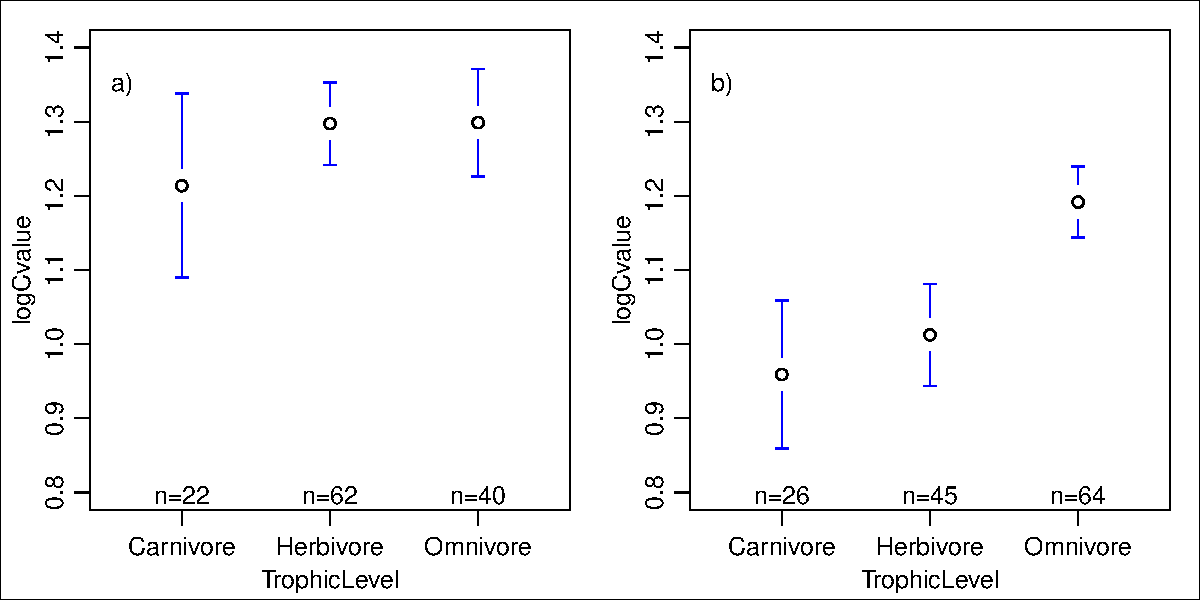
\includegraphics[width=0.9\textwidth]{plotmeans.pdf}

\caption{Means and 95\% confidence intervals for log genome size 
(picograms) in mammals for different trophic levels for a) ground 
dwelling species and b) other species.}

\label{fig:plotmeans}

\end{figure}

\begin{compactdesc}

\item [White space] The default options in R use wide margins and 
spaced out axes and take up a lot of space that could be used for 
plotting data. You've already seen the {\tt par} function and the 
options {\tt mfrow} for multiple plots and {\tt mar} to adjust margin 
size. The option {\tt mgp} adjusts the placement of the axis label, 
tick labels and tick locations. See {\tt ?par} for help on the these 
options.

\item [Main titles] Adding large titles to graphs is also a bad idea 
--- it uses lots of space to explain something that should be in the 
figure legend. With multiple plots in a figure, you have to label 
graphs so that the figure legend can refer to them. You can add labels 
using {\tt text(x,y,'label')}.

\item [Figure legends] A figure legend should give a clear stand-alone 
description of the whole figure. 

\item [Referring to figures] You {\it must} link from your text to 
your figures --- a reader has to know which figures refer to which 
results. So: `There are clear differences in mean genome size between 
species at different trophic levels and between ground dwelling and 
other species (Figure \ref{fig:plotmeans})'. 

\end{compactdesc}

\begin{compactitem}[$\quad\star$]
	
	\item Use {\tt plotmeans} from Chapter~\ref{ch:ANOVA} and the {\tt 
	subset} option to generate the two plots below. You will need to set 
	the {\tt ylim} option for the two plots to make them use the same $y$ 
	axis.
	
	\item Use {\tt text} to add labels --- the command {\tt par('usr')} 
	will show you the limits of the plot ($x_{min}, x_{max}, y_{min}, 
	y_{max}$) and help pick a location for the labels.

	\item Change the {\tt par} settings in your code and redraw the plots 
	to try and make better use of the space. In the example below, the 
	box shows the edges of the R graphics window.

\end{compactitem}
 
\section{Multiple explanatory variables}

All those graphs suggest:
\begin{compactitem}
 \item Carnivores have smaller genome size; omnivores have larger genome size. 
 \item Herbivores are somewhere in between, but not consistently.
 \item All ground dwelling mammals typically have larger genome sizes.
\end{compactitem}

We suspected these things from Chapter \ref{ch:ANOVA}, but now we can see 
that they might have separate effects. We'll fit a linear model to 
explore this and add the two explanatory variables together.
  
\begin{compactitem}[$\quad\star$]
\item This is an important section --- read it through carefully and 
ask questions if you are unsure. Copy the code into your script and add 
comments. {\it Do not just jump to the next action item}!
\end{compactitem}

\begin{lstlisting}
> model <- lm(logCvalue ~ TrophicLevel + GroundDwelling, data = mammals)	
\end{lstlisting}

We're going to do things right this time and check the model 
diagnostics before we rush into interpretation.

\begin{lstlisting}
> par(mfrow=c(2,2))
> plot(model)
\end{lstlisting}

\begin{center}
	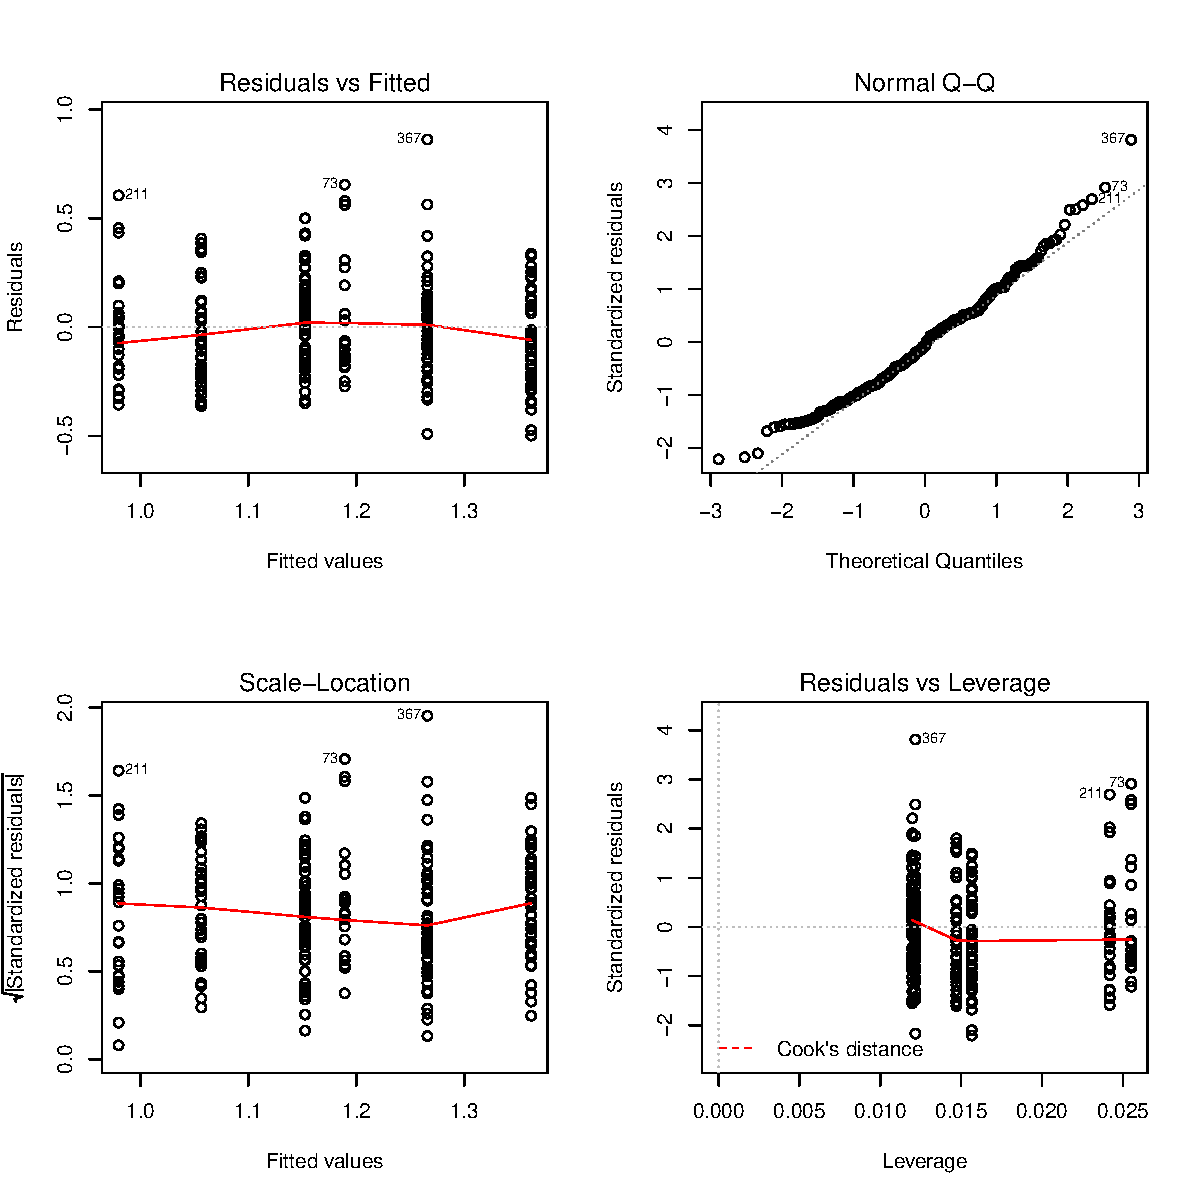
\includegraphics[width=\textwidth]{diagnostics1.pdf}
\end{center} 

There are six predicted values now - three trophic levels for each of 
the two levels of ground dwelling. Those plots look ok so now we can 
look  at the analysis of variance table:

\begin{lstlisting}
> anova(model)

 Analysis of Variance Table
 
 Response: logCvalue
                 Df Sum Sq Mean Sq F value  Pr(>F)    
 TrophicLevel     2   0.81   0.407    7.86 0.00049 ***
 GroundDwelling   1   2.75   2.747   53.04 4.1e-12 ***
 Residuals      255  13.21   0.052                    
 ---
 Signif. codes:  0 '***' 0.001 '**' 0.01 '*' 0.05 '.' 0.1 ' ' 1 
\end{lstlisting}

{\it Ignore the $p$ values}! Yes, they're highly significant but we 
want to understand the model, not rubber stamp it with `significant'.

\begin{compactitem}

 \item The sums of squares for the variables are both small compared to 
 the residual sums of squares --- there is lots of unexplained 
 variation. We can calculate the $r^2$ as explained sums of squares 
 over total sums of squares:
\[\frac{0.81 + 2.75}{0.81 + 2.75 + 13.21} = \frac{3.56}{16.77} = 0.212\]
 
\item Trophic level explain much less variation than ground dwelling 
--- this makes intuitive sense from the plots since there are big 
differences between Figure \ref{fig:plotmeans}a and 
\ref{fig:plotmeans}b, but small differences within.

\item We could also calculate a significance for the whole model by 
merging the terms. The total explained sums of squares of $0.81 + 2.75 
=3.56$ uses $2+1 =3$ degrees of freedom, so the mean sums of squares 
for all the terms together is $3.56/3=1.187$. Dividing this by the 
residual mean square of 0.052 gives an F of $1.187 / 0.052 = 22.83$.

\end{compactitem}

Now we can look at the summary table to see the coefficients. 

\begin{lstlisting}
> summary(model) 

 Call:
 lm(formula = logCvalue ~ TrophicLevel + GroundDwelling, data = mammals)
 
 Residuals:
     Min      1Q  Median      3Q     Max 
 -0.4990 -0.1784 -0.0146  0.1250  0.8624 
 
 Coefficients:
                       Estimate Std. Error t value Pr(>|t|)    
 (Intercept)             0.9798     0.0354   27.68  < 2e-16 ***
 TrophicLevelHerbivore   0.0766     0.0397    1.93    0.055 .  
 TrophicLevelOmnivore    0.1727     0.0398    4.34  2.0e-05 ***
 GroundDwellingYes       0.2095     0.0288    7.28  4.1e-12 ***
 ---
 Signif. codes:  0 '***' 0.001 '**' 0.01 '*' 0.05 '.' 0.1 ' ' 1 
 
 Residual standard error: 0.228 on 255 degrees of freedom
 Multiple R-squared: 0.212,	Adjusted R-squared: 0.203 
 F-statistic: 22.9 on 3 and 255 DF,  p-value: 3.6e-13 
 
\end{lstlisting}

Starting at the bottom, {\tt summary} has again calculated $r^2$ for us 
and also an $F$ statistic for the whole model, which matches the 
calculation above. 

The other important bits are the four coefficients. The intercept is 
now the reference level for two variables: it is the mean for 
carnivores that are not ground dwelling. We then have differences from 
this value for being an omnivore or herbivore and for being ground 
dwelling. There is a big change in genome size associated with ground 
dwelling and omnivory and both of these have large effects sizes, each 
introducing about a 20\% difference in genome size from the non-ground 
dwelling carnivores. In contrast, herbivory makes a small difference 
--- about 8\%. Because the difference is small and the standard error 
is large, the $t$ value suggests that this difference might arise just 
be chance. Put another way, it isn't significant.

The table below shows how these four coefficients combine to give the 
predicted values for each of the group means.

\[\begin{array}{|r|rrr|}
\hline
	       & \textrm{Carnivore} & \textrm{Herbivore} & \textrm{Omnivore}\\
\hline
\textrm{Not ground} & {\it 0.98} = 0.98    & {\it 0.98  + 0.08} =1.06    & {\it 0.98 + 0.17} =1.15 \\
\textrm{Ground}     & {\it 0.98 + 0.21} = 1.19    & {\it 0.98  + 0.08   + 0.21} =1.27   & {\it 0.98 + 0.17  + 0.21} =1.36\\
\hline
\end{array}\]

\section{Predicted values}

Getting the model predictions by hand in this way is tedious and error 
prone. There is handy function called {\tt predict} which uses the 
model directly to calculate values. The default is to give you the 
prediction for each point in the original data, but you can also ask 
for specific predictions.

The first thing to do is to set up a small data frame containing the 
explanatory values we want to use. The variable names and the level 
name have to match {\it exactly}, so we'll use the {\tt levels} 
function to get the names. We want to look at all six combinations, so 
we'll use the {\tt rep} function to set this up. The {\tt each=2} 
option repeats each value twice in succession; the {\tt times=3} 
options repeats the whole set of values three times.

\begin{lstlisting}
# data frame of combinations of variables
> gd <- rep(levels(mammals$GroundDwelling), times = 3)
> print(gd)

 [1] "No"  "Yes" "No"  "Yes" "No"  "Yes"
 
> tl <- rep(levels(mammals$TrophicLevel), each = 2)
> print(tl)

  [1] "Carnivore" "Carnivore" "Herbivore" "Herbivore" "Omnivore"  "Omnivore" 

> predVals <- data.frame(GroundDwelling = gd, TrophicLevel = tl)

\end{lstlisting}

Now we have the data frame of values we want, we can use predict. As 
when we created log values, we can save the output back into a new 
column in the data frame.

\begin{lstlisting}
> predVals$predict <- predict(model, newdata = predVals)
> print(predVals)

   GroundDwelling TrophicLevel predict
 1             No    Carnivore  0.9798
 2            Yes    Carnivore  1.1892
 3             No    Herbivore  1.0563
 4            Yes    Herbivore  1.2658
 5             No     Omnivore  1.1524
 6            Yes     Omnivore  1.3619
\end{lstlisting}

\begin{compactitem}[$\quad\star$]
	\item These are in the same order as the bars from your barplot. Make 
	a copy of the barplot and arrows code and then add the code below to 
	generate the plot. 
\end{compactitem}

\begin{lstlisting}
> points(barMids, predVals$predict, col= ' red ' , pch=5)
\end{lstlisting}

\begin{center}
	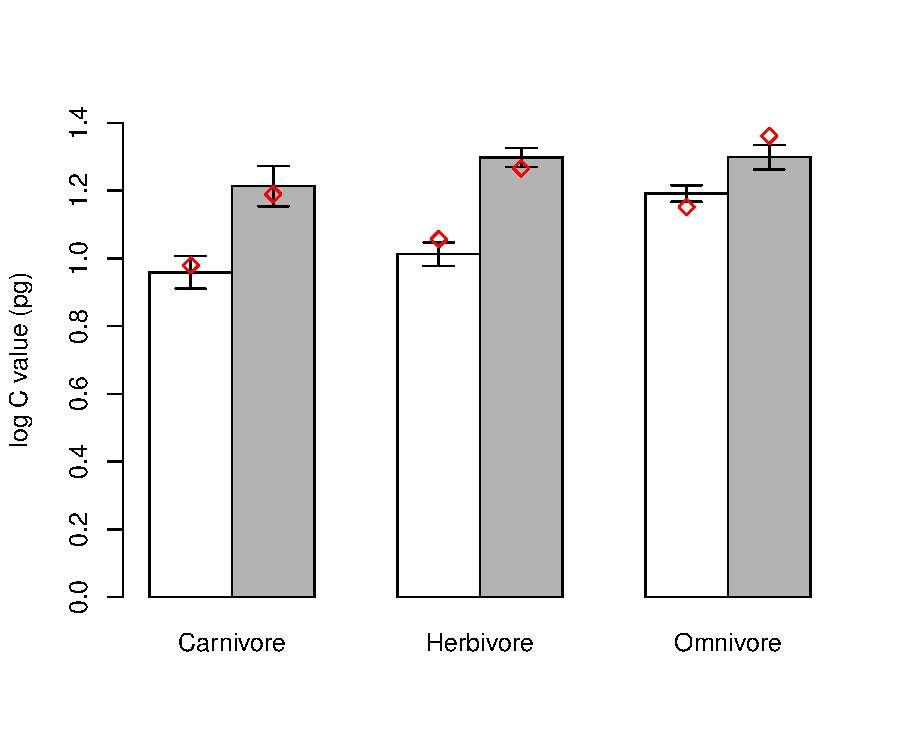
\includegraphics[width=0.6\textwidth]{barplotpred.pdf}
\end{center}

The red points do not match to the calculated means. This is because 
the model only includes a single difference between ground and 
non-ground species, which has to be the same for each trophic group. 
That is, there is no interaction between trophic level and ground / 
non-ground identity of each species in the current model.

The Chapter \ref{ch:MulExplInter} will look at interactions, which 
allows these values to differ using an interaction term in the model.
